\documentclass[essd, manuscript]{copernicus}

%% \usepackage commands included in the copernicus.cls:
%\usepackage[german, english]{babel}
%\usepackage{tabularx}
%\usepackage{cancel}
%\usepackage{multirow}
%\usepackage{supertabular}
%\usepackage{algorithmic}
%\usepackage{algorithm}
%\usepackage{amsthm}
%\usepackage{float}
%\usepackage{subfig}
%\usepackage{rotating}
\usepackage{amsmath}

\begin{document}

\title{Hector Permafrost}


% \Author[affil]{given_name}{surname}

\Author[1]{Dawn L.}{Woodard}
\Author[2]{Alexey N.}{Shiklomanov}
\Author[3]{Ben}{Kravitz}
\Author[4]{Corinne}{Hartin}
\Author[1]{Ben}{Bond-Lamberty}

\affil[1]{Joint Global Change Research Institute}
\affil[2]{Goddard Space Flight Center}
\affil[3]{Pacific Northwest National Laboratory}
\affil[4]{Environmental Protection Agency}
%% The [] brackets identify the author with the corresponding affiliation. 1, 2, 3, etc. should be inserted.

\correspondence{Dawn L. Woodard (dawn.woodard@pnnl.gov)}

\runningtitle{TEXT}

\runningauthor{TEXT}

\received{}
\pubdiscuss{} %% only important for two-stage journals
\revised{}
\accepted{}
\published{}

%% These dates will be inserted by Copernicus Publications during the typesetting process.


\firstpage{1}

\maketitle



\begin{abstract}
TEXT
\end{abstract}


\copyrightstatement{TEXT}


\introduction
Permafrost---soil that continuously remains below 0\degree C for at least two consecutive years---underlies an area of 22 ($\pm$ 3) million km$^2$, roughly 17\% of the Earth's exposed land surface \citep{gruber_2012_derivation}, and contains an estimated 1300 (1100-1500) Pg of organic carbon \citep{hugelius_2014_estimated}.
Recent increases in global air temperature \citep{ipcc_ar5_wg1}, which are amplified at high latitudes \citep{pithan_2014_arctic}, have resulted in widespread permafrost thaw \citep{romanovsky_2010_permafrost}, and simulations from variety of climate and land surface models across a wide range of scenarios suggest that this trend will continue into the future \citep{koven_2013_analysis; chadburn_2017_observation}.
Permafrost thaw can dramatically alter surface terrain and hydrology \citep{jones_2013_quantifying; godin_2014_effects; necsoiu_2013_multitemporal}, with adverse consequences for human infrastructure in permafrost regions \citep{anisimov_1997_permafrost; nelson_2002_climate; larsen_2008_estimating}.
Moreover, as permafrost thaws, this carbon becomes available to microbes for decomposition, resulting in the production of CO$_2$ and CH$_4$ \citep{brown_2008_report; romanovsky_2010_thermal; bond-lamberty_2016_temperature} that could lead to further warming \citep{koven_2011_permafrost; schuur_2015_climate}. Accounting for this permafrost carbon-climate feedback generally increases projections of greenhouse gas concentrations and global temperatures (REFS) and increases estimates of the economic impact of climate change \citep{hope_2015_economic; yumashev_2019_climate; chen_2019_economic}.

The higher carbon emissions associated with warming-driven permafrost thaw may be offset by increases in primary productivity.
Some studies based on meteorological tower measurements of carbon flux and optical remote sensing suggest that high-latitude ecosystems (mainly tundra and boreal forest) remain carbon-neutral or are even a small net carbon sink \citep{mcguire_2012_assessment; welp_2016_increasing}.
However, other studies, based on different sets of flux measurements and airborne gas sampling, suggest that the high-latitude regions are a net carbon source \citep{belshe_2013_tundra; commane_2017_carbon; natali_2019_large}.
The uncertainty in the net high-latitude carbon flux may be driven by the heterogeneity of high-latitude landscapes in terms of vegetation cover, soil properties, topography, and many other factors known to affect both the rate of permafrost thaw and the subsequent carbon flux \citep{turetsky_2002_boreal; wickland_2006_effects; lund_2010_variability; james_2013_multidecadal; johnson_2013_permafrost; grant_2019_modeling1; grant_2019_modeling2}.
This uncertainty is also present in recent permafrost modeling studies \citep{burke_2017_quantifying; qian_2010_enhanced; ito_2016_impacts; harp_2016_effect}.

Land surface models are expensive to run, making it challenging to use them for uncertainty quantification and exploration of alternative policy scenarios.
Simple climate models are an alternative.
(More on simple climate models).
(More on permafrost in simple climate models).

Hector \citep{hartin_2015_simple; vega-westhoff_2019_impacts}.
In this study, we implement a simple representation of permafrost thaw and evaluate its consequences for global climate in Hector.


\section{Model Description: Hector}
Hector \citep{hartin_2015_simple; hartin_2016_ocean}.
Simple climate model.

(TODO: More details on terrestrial C cycle in Hector).
The default heterotrophic respiration ($R$) scheme for a pool $p$ (detritus or soil) in Hector:

\begin{equation*}
R_{p} = C_p \times f_p \times Q_{10} ^ \frac{T}{10} \\    
\end{equation*} 


\subsection{Hector Permafrost Submodel}
The general principle is that permafrost constitutes an additional reserve of soil carbon that, because it is frozen, is inaccessible to microbes. As permafrost thaws and some fraction of this carbon becomes accessible to microbes, it is transferred from the frozen permafrost pool to the standard soil C pool, where it is decomposed by Hector's standard decomposition routine.

Let $C_{pf}[t]$ be the permafrost C pool and $C_{s}[t]$ be the soil C pool at time $t$ (both in units of Pg C), and let $\Delta C_{pf}[t]$ be the change in the permafrost C pool at time $t$.
The C consequences of permafrost thaw can therefore be represented as:

\begin{align*}
&C_{pf}[t] = C_{pf}[t-1] - \Delta C_{pf}[t]\\
&C_{s}[t] = C_{s}[t] + \Delta C_{pf}[t]\\
\end{align*}

Let $C[0]_{pf}$ be the initial size of the permafrost C pool (Pg C) and $\Phi[t]$ be the fraction of permafrost remaining (in arbitrary area or volume units) at time $t$.
Assuming a uniform permafrost C density, $\Delta C_{pf}[t]$ can be expressed as:

\begin{equation*} 
\Delta C_{pf}[t] = \Delta \Phi[t] C_{pf}[t-1]\\
\end{equation*}

To a first approximation, $\Phi[t]$ is a function of air temperature ($T[t]_{air}$).
[Kessler (2015)][kessler] assume this relationship is linear.
However, because the permafrost area fraction is, by definition, bounded by zero (and 1\footnotemark), and because deeper permafrost thaws more slowly than shallow permafrost, we use the lognormal cumulative distribution function ($NCDF(\log(x) | \mu, \sigma)$) instead:

\footnotetext{Technically, permafrost area could increase in the case of cooling temperatures, and therefore the area fraction could be greater than 1. However, because even the most aggressive climate action scenarios show temperatures that stabilize above year 2000, we assume that permafrost area will never grow more than the starting value.}

\begin{equation*}
\Phi[t] = 1 - NCDF(\log(x) | \mu, \sigma)\\
\end{equation*}

where $\mu$ and $\sigma$ are model parameters whose values are described in the \textit{Configuration} section below.
The change in frozen fraction at a given time step, $\Delta \Phi[t]$, is given by:

\begin{equation*}
\Delta \Phi[t] = \Phi[t] - \Phi[t-1]\\
\end{equation*}

[kessler]: https://econpapers.repec.org/RePEc:lsg:lsgwps:wp219

\begin{figure}
    \centering
    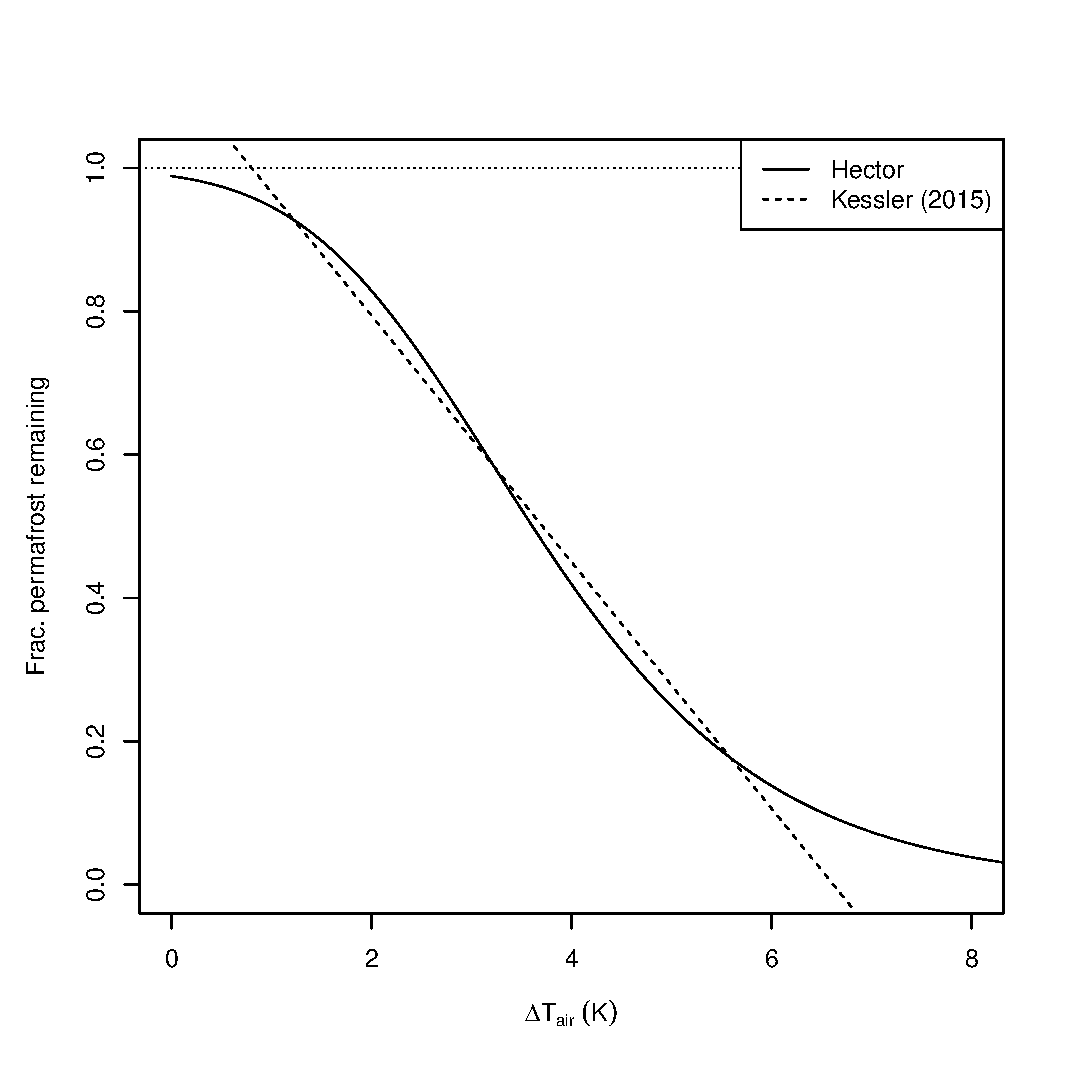
\includegraphics[width=0.8\textwidth]{figures/hector_vs_kessler.eps}
    \caption{REsults of turning on and off permafrost}
    \label{fig:4panel}
\end{figure}


\subsubsection{Methane Emissions}
In the default configuration of Hector, natural CH~4~ emissions are prescribed at a constant value (300 Tg year$^{-1}$) \citep{hartin_2015_simple}.
In the new configuration, CH$_4$ emissions are a fixed fraction of heterotrophic respiration.

Total heterotrophic respiration ($RH[i,t]$) for biome $i$ at time $t$ is the sum of heterotrophic respiration in detritus ($RH_d$) and soil ($RH_s$).

\begin{equation*} 
RH[i,t] = RH_s[i,t] + RH_d[i,t]
\end{equation*}

Detritus and soil heterotrophic respiration are proportional to the sizes of their respective carbon pools ($C_d$ and $C_s$, respectively, both in Pg C),
with a rate that increases exponentially with temperature according to a biome-specific temperature sensitivity parameter ($Q_{10}$).
Detritus respiration increases with biome-specific air temperature change since pre-industrial ($T[i,t]$),
while soil respiraiton increases with the 200 year running mean of air temperature ($T_{200}[i,t]$) because soils warm slowly relative to the atmosphere.

\begin{gather*}
T_{air}[i,t] = \delta T_{air}[t] \\
RH_d[i,t] = \frac{1}{4} C_d Q_{10}[i] ^ {{T}[i,t] / 10} \\
RH_s[i,t] = \frac{1}{50} C_s Q_{10}[i] ^ {T_{200}[i,t] / 10} \\
\end{gather*}

In the original formulation, natural CH~4~ emissions were a prescribed constant value.
In the revised version here, natural CH~4~ emissions are a fraction of heterotrophic respiration ($RH_{CH_4}[i,t]$) based on the biome-specific CH$^4$ fraction parameter ($f_{CH_4}[i]$):

\begin{equation*}
    RH_{CH_4}[i,t] = f_{CH_4}[i] RH[i,t] \\
\end{equation*}

\section{Configuration}
Initial permafrost C is set to 1035 Pg C based on the estimate for near-surface (<3 m depth) permafrost by \citet{hugelius_2014_estimated}.


For globally-averaged permafrost, exponential parameters $a = 2.371$, $b = -0.676$, and $c = -3.685$ to most closely reproduce the rate of 0.172 K$^{-1}$ reported by \citet{kessler_2017_estimating} over the range of 0.8 K \footnotemark to 4 K above the pre-industrial baseline.

\footnotetext{[Kessler (2015)][kessler] report this as temperature change from year 2000. 0.8 K is the warming since pre-industrial as estimated by the default Hector configuration.}

\section{Results}
Model demonstration of permafrost on and off
\begin{figure}
    \centering
    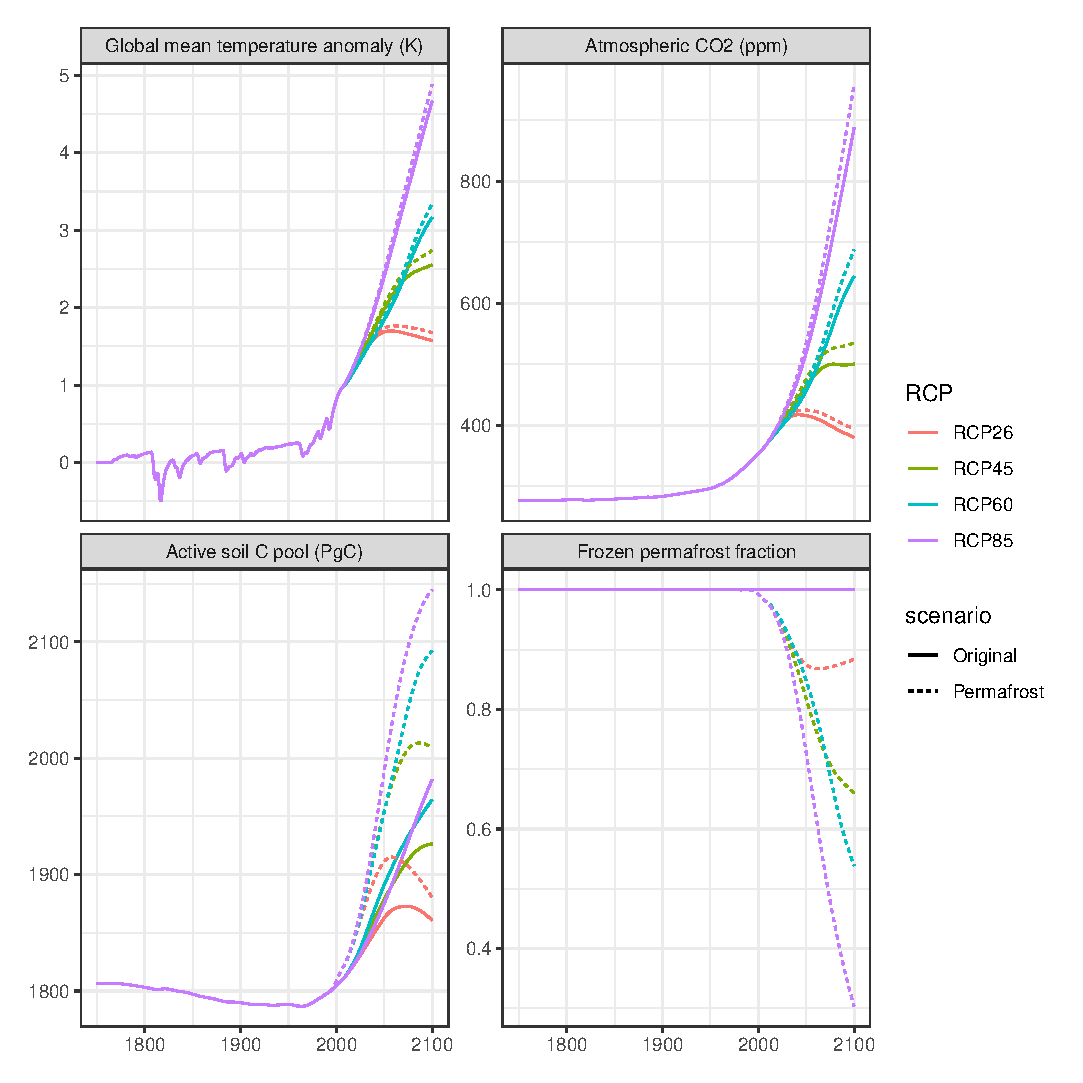
\includegraphics[width=\textwidth]{figures/hector_4panel_results.eps}
    \caption{REsults of turning on and off permafrost}
    \label{fig:4panel}
\end{figure}


Model sensitivity analysis

\section{Discussion}
Rate of permafrost C release also depends on soil moisture conditions -- drier soils release C much faster ("carbon bomb") than wetter soils ("carbon fizz") \citep{elberling_2013_long}.
Moisture will also affect the balance of aerobic (CO2 release) vs. anaerobic (CH4) C release \citep{turetsky_2002_boreal}, to the extent that unclear if anaerobic (wet) areas are C sources or sinks \citep{wickland_2006_effects}.
Effects of permafrost thaw on soil moisture are a complex hydrological problem -- drainage very sensitive to local (micro-)topography \citep{wickland_2006_effects}.
So will vegetation cover \citep{wickland_2006_effects}.

Temperature amplification of permafrost carbon feedback (by 2100) 0.02 to 0.36 °C \citep{burke_2013_estimating; schneider_2012_estimating; schneider_2015_observation}, or 0.1 to 0.8 °C in \citep{macdougall_2012_significant; macdougall_2013_if}, or 10-40\% of peak temperature change \citep{crichton_2016_permafrost}, or 0.2 to 12\% \citep{burke_2017_quantifying}.

Permafrost carbon has greater impact at lower emissions scenarios \citep{burke_2017_quantifying; @macdougall_2012_significant; @macdougall_2013_if} .


\conclusions  %% \conclusions[modified heading if necessary]
TEXT

%% The following commands are for the statements about the availability of data sets and/or software code corresponding to the manuscript.
%% It is strongly recommended to make use of these sections in case data sets and/or software code have been part of your research the article is based on.

\codeavailability{TEXT} %% use this section when having only software code available


\dataavailability{TEXT} %% use this section when having only data sets available


\codedataavailability{TEXT} %% use this section when having data sets and software code available


\sampleavailability{TEXT} %% use this section when having geoscientific samples available


\videosupplement{TEXT} %% use this section when having video supplements available


\appendix
\section{}    %% Appendix A

\subsection{}     %% Appendix A1, A2, etc.


\noappendix       %% use this to mark the end of the appendix section

%% Regarding figures and tables in appendices, the following two options are possible depending on your general handling of figures and tables in the manuscript environment:

%% Option 1: If you sorted all figures and tables into the sections of the text, please also sort the appendix figures and appendix tables into the respective appendix sections.
%% They will be correctly named automatically.

%% Option 2: If you put all figures after the reference list, please insert appendix tables and figures after the normal tables and figures.
%% To rename them correctly to A1, A2, etc., please add the following commands in front of them:

\appendixfigures  %% needs to be added in front of appendix figures

\appendixtables   %% needs to be added in front of appendix tables

%% Please add \clearpage between each table and/or figure. Further guidelines on figures and tables can be found below.



\authorcontribution{TEXT} %% this section is mandatory

\competinginterests{TEXT} %% this section is mandatory even if you declare that no competing interests are present

\disclaimer{TEXT} %% optional section

\begin{acknowledgements}
TEXT
\end{acknowledgements}




%% REFERENCES

\bibliographystyle{copernicus}
\bibliography{references.bib}
%%
%% URLs and DOIs can be entered in your BibTeX file as:
%%
%% URL = {http://www.xyz.org/~jones/idx_g.htm}
%% DOI = {10.5194/xyz}


%% LITERATURE CITATIONS
%%
%% command                        & example result
%% \citet{jones90}|               & Jones et al. (1990)
%% \citep{jones90}|               & (Jones et al., 1990)
%% \citep{jones90,jones93}|       & (Jones et al., 1990, 1993)
%% \citep[p.~32]{jones90}|        & (Jones et al., 1990, p.~32)
%% \citep[e.g.,][]{jones90}|      & (e.g., Jones et al., 1990)
%% \citep[e.g.,][p.~32]{jones90}| & (e.g., Jones et al., 1990, p.~32)
%% \citeauthor{jones90}|          & Jones et al.
%% \citeyear{jones90}|            & 1990



%% FIGURES

%% When figures and tables are placed at the end of the MS (article in one-column style), please add \clearpage
%% between bibliography and first table and/or figure as well as between each table and/or figure.


%% ONE-COLUMN FIGURES

%%f
%\begin{figure}[t]
%\includegraphics[width=8.3cm]{FILE NAME}
%\caption{TEXT}
%\end{figure}
%
%%% TWO-COLUMN FIGURES
%
%%f
%\begin{figure*}[t]
%\includegraphics[width=12cm]{FILE NAME}
%\caption{TEXT}
%\end{figure*}
%
%
%%% TABLES
%%%
%%% The different columns must be seperated with a & command and should
%%% end with \\ to identify the column brake.
%
%%% ONE-COLUMN TABLE
%
%%t
%\begin{table}[t]
%\caption{TEXT}
%\begin{tabular}{column = lcr}
%\tophline
%
%\middlehline
%
%\bottomhline
%\end{tabular}
%\belowtable{} % Table Footnotes
%\end{table}
%
%%% TWO-COLUMN TABLE
%
%%t
%\begin{table*}[t]
%\caption{TEXT}
%\begin{tabular}{column = lcr}
%\tophline
%
%\middlehline
%
%\bottomhline
%\end{tabular}
%\belowtable{} % Table Footnotes
%\end{table*}
%
%%% LANDSCAPE TABLE
%
%%t
%\begin{sidewaystable*}[t]
%\caption{TEXT}
%\begin{tabular}{column = lcr}
%\tophline
%
%\middlehline
%
%\bottomhline
%\end{tabular}
%\belowtable{} % Table Footnotes
%\end{sidewaystable*}
%
%
%%% MATHEMATICAL EXPRESSIONS
%
%%% All papers typeset by Copernicus Publications follow the math typesetting regulations
%%% given by the IUPAC Green Book (IUPAC: Quantities, Units and Symbols in Physical Chemistry,
%%% 2nd Edn., Blackwell Science, available at: http://old.iupac.org/publications/books/gbook/green_book_2ed.pdf, 1993).
%%%
%%% Physical quantities/variables are typeset in italic font (t for time, T for Temperature)
%%% Indices which are not defined are typeset in italic font (x, y, z, a, b, c)
%%% Items/objects which are defined are typeset in roman font (Car A, Car B)
%%% Descriptions/specifications which are defined by itself are typeset in roman font (abs, rel, ref, tot, net, ice)
%%% Abbreviations from 2 letters are typeset in roman font (RH, LAI)
%%% Vectors are identified in bold italic font using \vec{x}
%%% Matrices are identified in bold roman font
%%% Multiplication signs are typeset using the LaTeX commands \times (for vector products, grids, and exponential notations) or \cdot
%%% The character * should not be applied as mutliplication sign
%
%
%%% EQUATIONS
%
%%% Single-row equation
%
%\begin{equation}
%
%\end{equation}
%
%%% Multiline equation
%
%\begin{align}
%& 3 + 5 = 8\\
%& 3 + 5 = 8\\
%& 3 + 5 = 8
%\end{align}
%
%
%%% MATRICES
%
%\begin{matrix}
%x & y & z\\
%x & y & z\\
%x & y & z\\
%\end{matrix}
%
%
%%% ALGORITHM
%
%\begin{algorithm}
%\caption{...}
%\label{a1}
%\begin{algorithmic}
%...
%\end{algorithmic}
%\end{algorithm}
%
%
%%% CHEMICAL FORMULAS AND REACTIONS
%
%%% For formulas embedded in the text, please use \chem{}
%
%%% The reaction environment creates labels including the letter R, i.e. (R1), (R2), etc.
%
%\begin{reaction}
%%% \rightarrow should be used for normal (one-way) chemical reactions
%%% \rightleftharpoons should be used for equilibria
%%% \leftrightarrow should be used for resonance structures
%\end{reaction}
%
%
%%% PHYSICAL UNITS
%%%
%%% Please use \unit{} and apply the exponential notation


\end{document}
